\documentclass{IEEEtran}[11pt]
\usepackage{graphicx}
\usepackage{amsmath}
\usepackage[utf8]{inputenc}
\raggedbottom
\title{Using Normalised Radial Based Functions (NRBF's) to Predict Energy Consumption in the National Grid}
\author{Student Number : 10523192}
\date{11/01/2018}

\begin{document}
\pagenumbering{arabic}

\maketitle

%\tableofcontents
\newpage
\section{Introduction}
\begin{flushleft}
  Neural network used to forecast future events are very import and useful to
  modern life and computer science. Using these tool we can a good idea of
  future event and what effect it might have later on. For this paper an NRBF
  network will be used to try and predict energy consumption in the national grid
  for the year of 2017.
\end{flushleft}
\section{Network}
\subsection{NRBF}
\begin{flushleft}
  Normalised Radial Based Functions (NRBF) networks work by using the activation
  of all nodes in the hidden layer to work out the output of the network. This
  is done by using the Gaussian activation function of the nodes in the hidden
  layer, to work out how active each node is when a value is passed to that
  node in the hidden layer. If a node is very active then its activation value
  will be one or very close to one, where as an inactive node will be much
  closer to zero. The activation of all of the nodes is later used to work out
  what the output of the network will be.
\end{flushleft}

\begin{flushleft}
  When the activation has been calculated this can then be used to get the output of the network
  as the more active nodes will contribute more to the final value that is output based on these inputs.
  To do this the sum of the nodes weights multiplied by the activation of the node is calculated.
  This part of the equation can be seen in figure 1:
  \vspace{3mm}

  $$\sum_{n=1}^{N}W _n\phi(\|x-x_n\|) $$
  \\
  \vspace{1.5mm}

  {\footnotesize figure 1 : sum of all node activations multiplied by weights of all nodes}

  \vspace{3mm}
  After this the total sum of all node activations is calculated and summed.
  The equation for this can be seen figure 2.

  \vspace{3mm}

  $$\sum_{n=1}^{N}\phi(\|x-x_n\|) $$
  \\
  \vspace{1.5mm}

  {\footnotesize figure 2 : sum of all node activations}
  \\
  \vspace{3mm}
  When these have been calculated the 2 values are divided. to get the final
  output from the hidden layer. Then these values are passed to the output layer
  and the final network output is stored.
  The whole equation can been seen in figure 3.

  \vspace{3mm}

  $$f(x)=\frac{\sum_{n=1}^{N}W _n\phi(\|x-x_n\|)}{\sum_{n=1}^{N}\phi(\|x-x_n\|)}$$
  \\
  \vspace{1.5mm}

  {\footnotesize figure 3 : sum of all node activations multiplied by weights of all nodes
  divided by sum of all node activations}
  \\
  \vspace{3mm}

\end{flushleft}

\begin{center}
  Node Activation Equation
\end{center}
\begin{flushleft}
  The node activation equation is used to calculated how activation a node in
  the hidden layer is when being given a set of inputs. If the value before
  the exponential is calculated is 0 then the activation value of the node
  will be 1. This equation can be seen in figure 4.
\end{flushleft}
$$y=exp(-\frac{1}{2\sigma^2} \sum_{k=1}^{K}(x_{k} - w_{jk})^2) $$
{\footnotesize figure 4 : Gaussian activation equation for NRBF nodes}
\begin{center}
  Root Mean Squar Equation
\end{center}
\begin{flushleft}
  The Root Mean Square equation is used to calculated how the network preformed
  on the data sets it was being shown. This value can then be used to determine
  the best number of nodes and best sigma values for the network.
\end{flushleft}
$$RMS =\sqrt{\frac{1}{M}\sum_{i=1}^{M}(y^{p}_{i} - y^{p}_{id})^2} $$
{\footnotesize figure 5 : Root Mean Square equation for calculating the error of the network}
\begin{center}
  Weight Update Equation
\end{center}
\begin{flushleft}
  The weight update equation is used to adjust the weights of the nodes in the
  hidden layer.
  This will allow the network to become more accurate over time as the weights
  get adjusted closer to there optimal values, as the network becomes more
  accurate these adjustments become smaller. To do this the old weight is
  added to using the learning rate ($\alpha$) multiplied by the target value
  - the networks output, this is then multiplied by the activation of the node
  ($\phi$).
\end{flushleft}
$$ W  \leftarrow W + \alpha *(target - Network output)*\phi$$
{\footnotesize figure 6 : Weight update equation used in the NRBF}

\subsubsection{Task 1}
\begin{flushleft}
  For task one an NRBF was made to work on a small and evenly distributed data
  set, to get the understanding of the network and the maths that would be used.
  To make sure the network was working correctly the sigma was set to 0.01 to
  see the step of the network function. This can be seen in figure 7. This was
  useful as it allowed to check if the network was working and was covering all
  of the training data points with the network function.
  \vspace{1.5mm}
  \\
  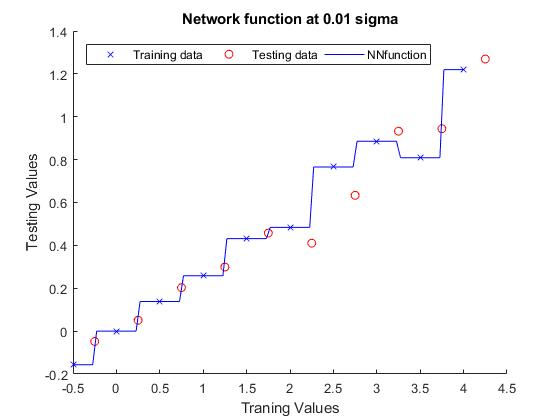
\includegraphics[width = 0.45\textwidth]{NNstepfunction.jpg}
  \\
  \vspace{1.5mm}
  {\footnotesize figure 7 : Network function when sigma is 0.01 }
  \\
  \vspace{1.5mm}
  Once the network was working properly, the sigma optimisation could begin to
  see which sigma would be best to use for the network. To do this the network
  was run over the data set 100 times and then the best test and train error
  where taken and stored. This allowed for the best value on the testing data to
  be found. The sigma was tested between 0.1 - 1 and the table of results can be
  seen in figure 10. The best sigma value that could be found from this testing
  was 0.9 as it had the lowest test error of all of the value tried with a error
  value of 0.0915. The error graph and network function graph for this sigma
  can be seen in figure 8 and 9.
  \\
  \vspace{1.5mm}
  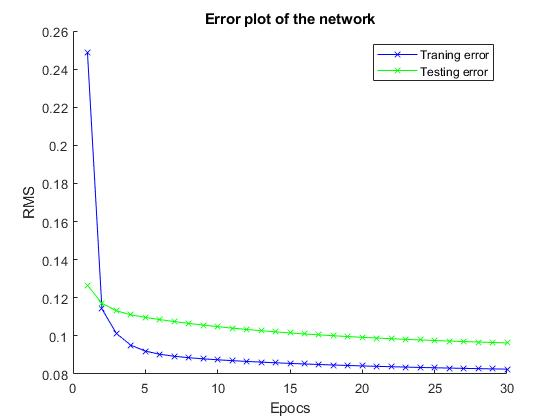
\includegraphics[width = 0.45\textwidth]{Errorplottask1.jpg}
  \vspace{1.5mm}
  {\footnotesize figure 8 : error plot for the network with sigma 0.9 }
  \\
  \vspace{1.5mm}
  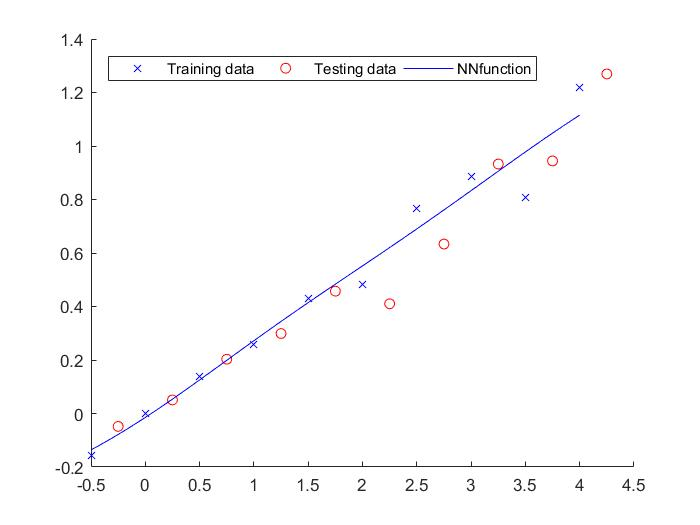
\includegraphics[width = 0.45\textwidth]{NNfunctiontask1.jpg}
  \vspace{1.5mm}
  {\footnotesize figure 9 : Network function when sigma is 0.9 }
  \\
  \vspace{1.5mm}
\end{flushleft}
\begin{center}
  \begin{tabular}{||c c c||}
    \hline
    Sigma Value & Train Error & Test Error \\ [0.5ex]
    \hline
    0.1 & 0.2733e-16 & 0.1005\\
    0.2 & 2.0126e-10 & 0.1016\\
    0.3 & 1.3562e-4 & 0.1094\\
    0.4 & 0.0131 & 0.1161 \\
    0.5 & 0.0439 & 0.1073 \\
    0.6 & 0.0632 & 0.0983\\
    0.7 & 0.0730 & 0.0933\\
    0.8 & 0.0781 & 0.0919\\
    0.9 & 0.0797 & 0.0915\\
    1.0 & 0.0800 & 0.0918\\
    \hline
  \end{tabular}
\end{center}
\vspace{1.5mm}
{\footnotesize figure 10 : Sigma optimisation table }
\\
\vspace{1.5mm}
\subsubsection{Tast 2}

\begin{flushleft}
  For task 2 a NRBF that could predict the output of the national grid need to
  be made. This network would be much larger and more complex then the first one
  due to the fact that more data points would exist. When first creating and
  testing the network a node was used for each data point to check that every
  thing was working correctly, but this was not the best practice as some data
  points where very similar and could fit under one NRBF node.
  \\
  \vspace{2.5mm}
  So to lower the amount of nodes used in the hidden layer but still ensure
  that the nodes where evenly distributed K-means clustering was use to separate
  the data in to sets of clusters and then create the node centres. This meant
  that the number of nodes used would always be able cover the whole data set.
  This then allowed for testing in the form of node optimisation and sigma
  optimisation to get a much more efficient network. To get the number of nodes
  the total size of the data set is divided by a set number and that many nodes
  centres are then created. These node centres then used to set the centres of
  each node. As this network is a 3 dimensional network each node will be given
  3 centres and have 3 input weight.
  \\
  \vspace{2.5mm}
  After the nodes have been created the input values are looped through by the
  network and each one is tested. After a data point has been passed through the
  network the weights are updated and another data point is passed through the
  network, after all the data point have been tested another epoc is run going
  through the data points again. This is done 100 times to allow for the larger
  sigma's to be trained by the network. The years 2012-2015 are used to train
  the network then the 2016 data set is used for testing the network. 2017 data
  set is used to validate the network performance.
  \\
  \vspace{2.5mm}
  The network was trained across all of the training sets to allow for the network
  to be trained on all of the data available over those years and tested after
  each epoc. To ensure that the network was fully prepared for the final
  validation data set.
  \\
  \vspace{1.5mm}
  The graphs for all of this can be seen in the results section of this report
  \\
  \vspace{1.5mm}
  When optimising the network a number of different nodes and sigmas where
  tested to achieve the best possible value for the final network. this was done
  by testing each node combination chosen on each sigma value between 0.1 - 1.
  This allowed for each sigma to be collected and then compared, the best sigmas
  for each node combination chosen can be seen in figure 11.
  \\
  \vspace{1.5mm}
  From doing this the optimal nodes seemed to be 8724 which is very close to 1
  node per data point in the data set, then the optimal sigma value was 0.1 as
  it had the lowest test error of any of the sigmas this can be seen in
  figure 12. After the optimal amount of nodes and sigma was found the network
  was passed the validation data to see what the networks prediction would look
  like.
  \\
  \vspace{1.5mm}
\end{flushleft}
  \begin{center}
    \begin{tabular}{||c c c c||}
      \hline
      Nodes & Best Sigma & Train Error & Test Error \\ [0.5ex]
      \hline
      8724 & 0.1 & 0.0165 & 0.0282 \\
      4380 & 1 & 0.0482 & 0.0687 \\
      2190 & 1 & 0.0482 & 0.0688 \\
      1095 & 0.9 & 0.0472 & 0.0678\\
      547  & 0.9 & 0.0471 & 0.0679\\
      237  & 0.8 & 0.0446 & 0.0687\\
      136  & 0.9 & 0.0474 & 0.0681\\
      68   & 0.9 & 0.0475 & 0.0680\\
      \hline
    \end{tabular}
    \\
    \vspace{2.5mm}
    {\footnotesize figure 11 : Number of nodes compared to training error and
    test error}
    \\
    \vspace{2.5mm}
  \end{center}
\begin{center}
  \begin{tabular}{||c c c||}
    \hline
    Sigma Value & Train Error & Test Error \\ [0.5ex]
    \hline
    0.1 & 0.0165 & 0.0282 \\
    0.2 & 0.0187 & 0.0334 \\
    0.3 & 0.0250 & 0.0432 \\
    0.4 & 0.0332 & 0.0701 \\
    0.5 & 0.0362 & 0.0733 \\
    0.6 & 0.0386 & 0.0747 \\
    0.7 & 0.0393 & 0.0708 \\
    0.8 & 0.0443 & 0.0695 \\
    0.9 & 0.0472 & 0.0690 \\
    1.0 & 0.0482 & 0.0686 \\
    \hline
  \end{tabular}
  \\
  \vspace{2.5mm}
  {\footnotesize figure 12 : Sigma optimisation of nodes the network based on the
  best number of nodes}
\end{center}
\subsection{MLP}
\subsubsection{Task 2}
\begin{flushleft}
  MLP or Multi Layer Perceptron are a form of neural network that use sigmod activations
  to get an output based on all of the nodes in the hidden layer. Unlike NRBFS nodes in
  MLP's nodes don't have centres, and instead each node weight value is used to get a
  part of the final output. To get an output value from the network the sigmod activation
  is calculated from the input to the hidden layer. Then the hidden layer sigmod activation
  is calculated and passed to the output layer, where the total activation of all hidden
  nodes is calculated leading to the network output. The sigmod activation
  equation can be seen in the figure 13.
  \\
  \vspace{1.5mm}
  To optimise the MLP the number of nodes can be changed to see how this affects
  the overall output of the network. This can have a drastic change on the
  performance of the network, as the more nodes that are there the larger the
  impact the hidden node will have on the final network output. This has some
  problems as the nodes in the hidden layer will all be updated when the back
  propagation on the network takes place meaning that each node will be moved
  slightly based on the final output. This means that the MLP can never be 100\%
  accurate as its value is shifted every time so its best on the value that it
  has previously seen.

  $$y_i=\frac{1}{1+exp(-z_i)}$$
  \\
  \vspace{1.5mm}
  {\footnotesize figure 13 : Sigmod activation function used in the MLP}
  \\
  \vspace{1.5mm}
  When updating the weights in the network the delta rule is used to update all of
  the weights in the network. This works by taking the weight value and adding
  the learning rate multiplied by the target value take the networks out put.
   the equation for this can be seen in figure 14.
  $$W \leftarrow W  + \alpha*(y_i,_d - y_i)$$
  {\footnotesize figure 14 : Delta rule weight update equation where $\alpha$ is the learning
  rate}
  \\
  \vspace{1.5mm}

  To optimise this network the max number of nodes was used and records of the
  error on training and testing data was monitored and the number of nodes was
  slowly decreased over different tests to see which amount of nodes would yield
  the best results. From this the best amount of nodes for the MLP where in the
  range of 30-40 as these all had the same error value of 0.0577 with a learning
  rate of 0.01.
  \\
  \vspace{1.5mm}
  Along with this the learning rate was changed to see how this can affect the
  performance of the MLP. This lead to a large improvement in the network
  performance but still did not out preformed the NRBF network. The MLP seems to
  be able to get it's output values around the right values but is still very
  far off the correct answer.
  \\
  \vspace{1.5mm}
  From looking at the node and learning rate optimise tables in figure 15 \& 16
  it shows that the best number of nodes and learning rates are 31 nodes with a
  learning rate ($\alpha$) 0f 0.01. This node and learning rate values where
  found after testing the learning rate of 0.2 but found this to be to high, so
  a range of values between 0.1- 0.01 where tested on these number of nodes
  to see how this affected the networks output. The prediction from the MLP can
  be seen in the Results section of the report.

  \begin{center}
    \begin{tabular}{||c c c||}
      \hline
      Nodes & $\alpha $ & Test Error \\ [0.5ex]
      \hline
      1000 & 0.05 & 0.0631 \\
      500 & 0.01 &  0.0609 \\
      250 & 0.01 & 0.0614 \\
      125 & 0.01 & 0.0586\\
      62  & 0.05 & 0.0634\\
      31  & 0.01 & 0.0577\\
      \hline
    \end{tabular}
    \\
    \vspace{2.5mm}
    {\footnotesize figure 15 : best learning rate for each node amount tested on
    the MLP}
    \\
    \vspace{2.5mm}
  \end{center}
\begin{center}
  \begin{tabular}{||c c c||}
    \hline
    Nodes & $\alpha $  & Test Error \\ [0.5ex]
    \hline
    1000 & 0.01 & 0.0660 \\
    500 & 0.01 &  0.0609 \\
    250 & 0.01 & 0.0614 \\
    125 & 0.01 & 0.0586\\
    62  & 0.01 & 0.0650\\
    31  & 0.01 & 0.0577\\
    \hline
  \end{tabular}
  \\
  \vspace{2.5mm}
  {\footnotesize figure 16 : all node test error after the best learning rate
  had been identified}
\end{center}
\end{flushleft}
\section{Data}
\subsection{Data processing methods}
\begin{flushleft}
  along with the day of the year, hour of day and the day of the week. This data
  was then normalised to be used in the network, to normalised the day the value
  would be divided by 365. For example the first day of the year would be
  $1 / 365$. To normalised the hour of the day was taken and then divided by 24
  to get the normalised value. Finally the day of the week was divided by 7 to
  get a normalised set of numbers between 0 and 1. The data was then set up in
  the file to be in the format of : Day of year, Hour of day , Day of week,
  Arrearage demand
  \\
  \vspace{1.5mm}
  Along with this the data processing could not factor in some of the data in
  the file, like the large spikes that occur from time to time and the leap
  years that also occur. These could of been factor in but then would also would
  of need to be factored in to the network when training leading to more problems.
\end{flushleft}
\subsection{Problems with the data}
\begin{flushleft}
  When processing the data there was a large array of problems that occurred.
  Some of the years of data where not complete and where missing entries over
  the year, 2016 even contained reading that where abnormally low. This was most
  likely a miss reading or problem with the equipment that is used for the
  reading but this will still cause massive problems for network when it
  comes training. Along with this the data reading where not always evenly sampled
  meaning some reading are very close to other where as others are very spaced apart.
  This is a very large problem when it comes to training to make the network as
  accurate as possible as the data might not reflect the height demands that
  could of occurred during the time of the reading. Along with this the data is
  sampled every 5 minutes, so to make the network as accurate as possible data
  would need to be taken more frequently and used to train the network.
  \\
  \vspace{1.5mm}
  With some years be leap years this leads to the problem of there being 1
  extra day for the network to learn that is not consistently there every year.
  This could be factored in to the network but would most likely only make a
  miner changer to the networks performance. Along with this there are spikes in
  the data where large world events had taken place or large sports events had
  taken place, this meant that more power was need and used as a result.
  This could be factored in to the network but there are so many edge cases and
  events that can not be predicted that it would most likely hinder rather then
  help the network to learn. Along with this cancelation of events or events only
  running every few years e.g. the Olympics would also need to be factored in
  and might lead to more energy being in the grid then is need. examples of the
  spikes can be seen in figure 17.
  \vspace{1.5mm}
  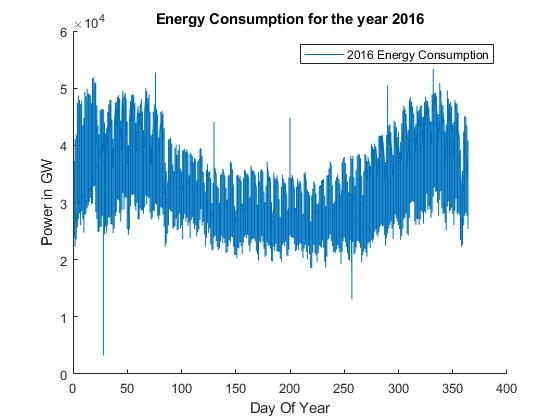
\includegraphics[width = 0.45\textwidth]{2016datasetplotted}
  \vspace{1.5mm}
  {\footnotesize figure 17 : Plot of hourly energy consumption over 2016}
  \\
  \vspace{1.5mm}

\end{flushleft}
\section{results}
\begin{flushleft}
  The results from the NRBF after being trained across the 2012-2015 data was
  very interesting as the network seemed to have a better prediction then expected.
  The network seems to over predict the amount of energy required in the national
  grid at most of the times of year and seems to not fit the data at the bottom
  end of the data set along with this it struggles to predict the  lower energy
  consumption in the summer month.
  \\
  \vspace{1.5mm}
  The network over predicts the energy consumption
  at the start of the summer months around day 150 and then fails to predict the
  lower energy periods around day 175 - 200. Along with this it seems to struggle
  predicting the higher energy consumption that took place at the end of the year
  around mid to late December, this may be due to the fact that 2017 might have
  had higher energy consumption then previous December's.
  \vspace{1.5mm}
  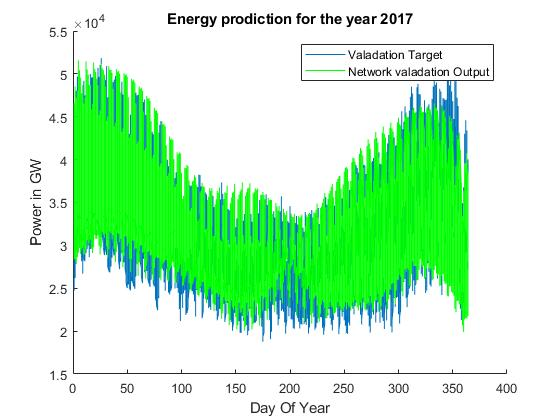
\includegraphics[width = 0.45\textwidth]{2017prediction.jpg}
  \vspace{1.5mm}
  {\footnotesize figure 18 : NRBF prediction of the energy consumption over the
  year of 2017 }
  \\
  \vspace{1.5mm}

  To achieve even better results the network could of been tested across 2dp sigmas
  to see how this would affect the over all prediction that the network would
  make in the end. Also the learning rates could be changed and tested to
  see how the network would change in term of its final prediction.
  \\
  \vspace{1.5mm}
  While testing the network a plot of the network function was made to see how
  the network was fitting the data set. This showed the network was over fitting
  to the data set that it was using, but still yielded the best results across
  all of the node and sigma optimisation that was preformed. Along with this the
  network seemed to still have not learned the peaks that occur in the data set
  reinforcing the idea the network could not learn this data easily.
  \\
  \space{1.5mm}
  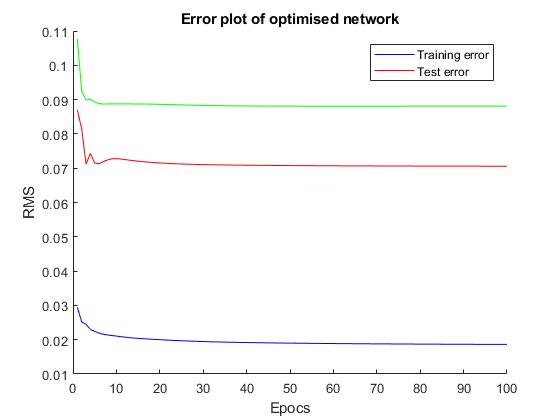
\includegraphics[width = 0.45\textwidth]{errorPrediction.jpg}
  \vspace{1.5mm}
  {\footnotesize figure 18 : Error plot of the network on training data, test data
  and validation data.
  year of 2017 }
  \\
  \vspace{1.5mm}
  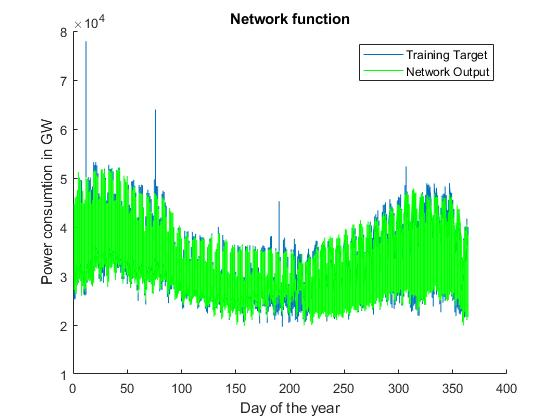
\includegraphics[width = 0.45\textwidth]{predictiontrainingdata.jpg}
  \vspace{1.5mm}
  {\footnotesize figure 19 : Plot of the network output on training data set }
  \\
  \vspace{1.5mm}

  The results from the MLP are no where near as accurate as the NRBF result
  the MLP seemed to not be able to see the different in energy fluctuation
  in the data set and only trends downwards over the year. This again shows
  that this type of network is not suited for forecasting type tasks. The
  prediction of the MLP can be seen in figure 20.
  \\
  \vspace{1.5mm}
  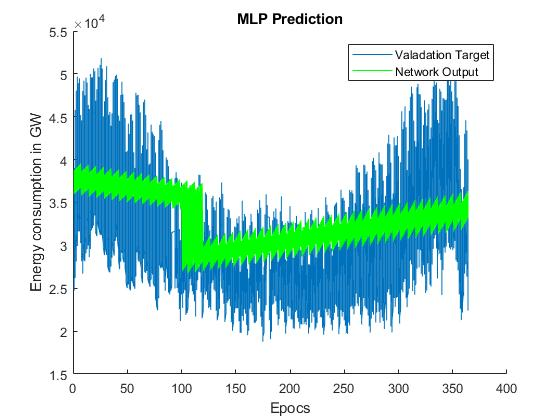
\includegraphics[width = 0.45\textwidth]{MLPprediction.jpg}
  \vspace{1.5mm}
  {\footnotesize figure 20 : MLP prediction }
  \\
  \vspace{1.5mm}
  Comparing the Prediction to the network function, they are both very similar
  and seem to be just a larger network function. This helps to show that the
  network is not over fitting like the NRBF which might be contributing to the
  fact that its prediction is not as good. Along with this you can see how the
  network seems to be preforming worse on the validation data as the epocs go on
  while the train and test error trend down ward. This can be seen in figure 21.
  \\
  \vspace{1.5mm}
  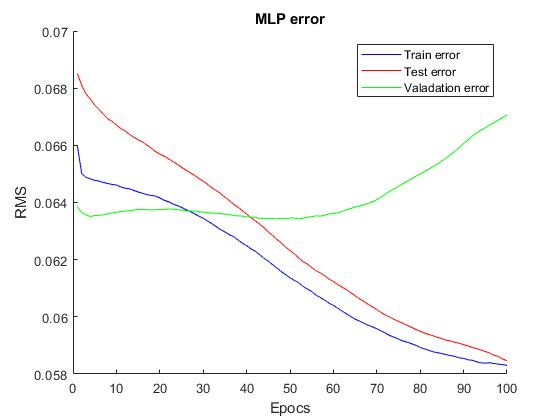
\includegraphics[width = 0.45\textwidth]{MLPerrorPlot.jpg}
  \vspace{1.5mm}
  {\footnotesize figure 21 : MLP error plot }
  \\
  \vspace{1.5mm}
  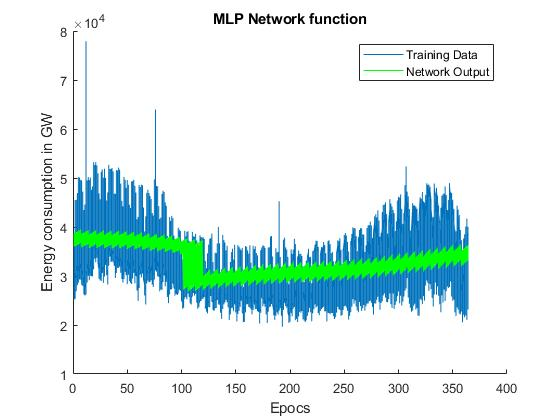
\includegraphics[width = 0.45\textwidth]{MLPNetworkFunction.jpg}
  \vspace{1.5mm}
  {\footnotesize figure 22 : MLP Network function }
\end{flushleft}

\section{conclution}
\begin{flushleft}
  With all the information and results gather through out this project it shows
  how an NRBF networks can be used to forecast future events with enough data and
  training. The results are not perfect, but they seem to out preform MLP's on the
  same type of task. To improve the network further more sigma optimisation
  could be carried out to try and get a sigma to 2dp, as this could greatly increase
  the performance of the network. If there was more time and the task could be
  moved to parallel computation methods then testing each sigma value from 0.1
  - 1 could also be carried out more to work out the average across 100 trials to
  help conform the results of the best sigma and nodes. This would also allow
  for testing across larger epoc amounts.
  \\
  \vspace{1.5mm}
  The data processing method that was used was not the best and could of been
  improved on to get slightly more accurate results and data to be feed in to
  the network. With this some more work could of been done to improve the MLP
  and different architecture and even multiple layers could be used to improve
  the performance of the MLP. The MLP could also of been paralysed to allow for
  the training and optimisation of nodes and learning rates to be speed up and
  covered across larger node amount and a larger range of learning rates.
  \\
  \vspace{1.5mm}
  The NRBF can also be tested against new form of
  networks to see how it compares to the likes of Convolutional or spikey
  neural network, to see how it compares to there Prediction.
  \\
  \vspace{1.5mm}
  Finally the network could also be trained differently to see how this affect
  the final out come. The network could be trained using all of the data sets
  in one go rather then having them split up over each year, and also could
  trained using decaying learning rates as the network starts to preform better
  on the data sets. This might help to avoid over fitting on the final data set.
\end{flushleft}
\end{document}
